\section{Dynamische Preisgenerierung}
\label{subsec:revpar_price}
Durch die Implementierung des Modells in der vorherigen Sektion werden normierte RevPAR-Werte generiert, die in einem DataFrame wie folgt dargestellt werden können:

\begin{figure}[h]
    \centering
    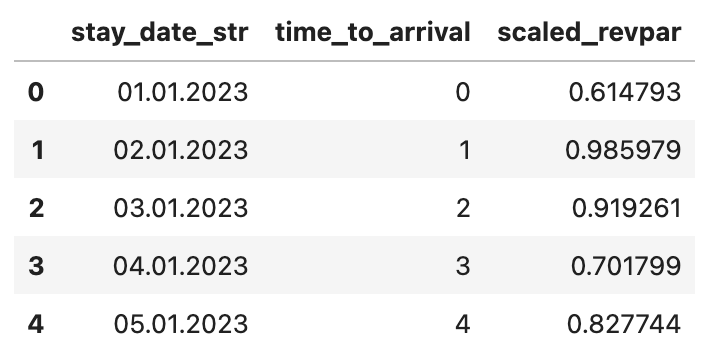
\includegraphics[width=1\textwidth, center]{revpar_price_1.png}
    \caption[Datensatz der Vorhersage]{Datensatz der Vorhersage}
    \label{img:revpar_price_1}
\end{figure}

Um die tatsächlichen Preise unter Verwendung des RevPAR-Preis-Mappings für die einzelnen Zimmerkategorien zu generieren, ist es erforderlich, die normierten RevPAR-Werte in ihre ursprüngliche Form zu überführen. Dies erfolgt durch die Multiplikation der normierten RevPAR-Werte mit dem durchschnittlichen RevPAR-Wert des Hotels. Zu diesem Zweck wird dem DataFrame eine zusätzliche Spalte mit dem Namen \emph{revpar} hinzugefügt. Diese Spalte repräsentiert das Produkt aus dem normierten RevPAR und dem durchschnittlichen RevPAR des Hotels.

\begin{figure}[h]
    \centering
    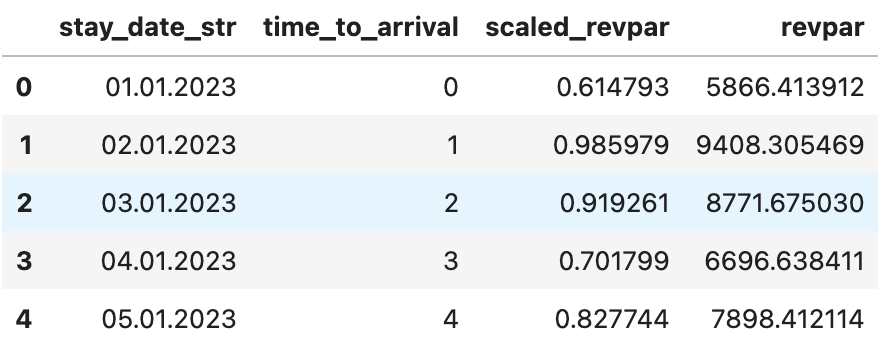
\includegraphics[width=1\textwidth, center]{revpar_price_2.png}
    \caption[Datensatz mit dem tatsächlichen RevPAR-Werten]{Datensatz mit dem tatsächlichen RevPAR-Werten}
    \label{img:revpar_price_2}
\end{figure}

Durch diese Vorgehensweise wurde eine vergleichbare Ausgangssituation wie beim ursprünglichen RevPAR-Modell geschaffen. Von diesem Punkt an kann das Mapping vom RevPAR-Wert zum Preis verwendet werden, um die tatsächlichen Zimmerpreise zu generieren.
\newpage
\begin{figure}[h]
    \centering
    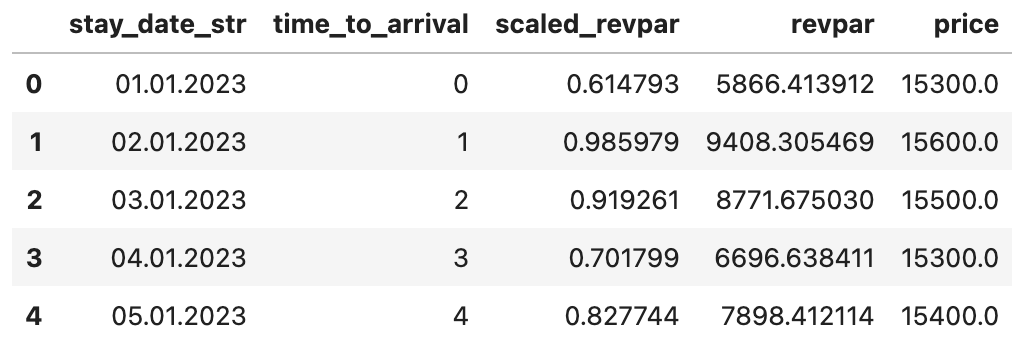
\includegraphics[width=1\textwidth, center]{revpar_price_3.png}
    \caption[Datensatz mit dem tatsächlichen Preisen]{Datensatz mit dem tatsächlichen Preisen}
    \label{img:revpar_price_3}
\end{figure}

Die Abbildung \ref{img:revpar_price_3} zeigt beispielhaft die Preise in Cent für eine bestimmte Zimmerkategorie, die schließlich dem Kunden vorgeschlagen werden.